\documentclass{ximera}

%\usepackage{todonotes}

\newcommand{\todo}{}

\usepackage{esint} % for \oiint
\ifxake%%https://math.meta.stackexchange.com/questions/9973/how-do-you-render-a-closed-surface-double-integral
\renewcommand{\oiint}{{\large\bigcirc}\kern-1.56em\iint}
\fi


\graphicspath{
  {./}
  {ximeraTutorial/}
  {basicPhilosophy/}
  {functionsOfSeveralVariables/}
  {normalVectors/}
  {lagrangeMultipliers/}
  {vectorFields/}
  {greensTheorem/}
  {shapeOfThingsToCome/}
  {dotProducts/}
  {partialDerivativesAndTheGradientVector/}
  {../productAndQuotientRules/exercises/}
  {../normalVectors/exercisesParametricPlots/}
  {../continuityOfFunctionsOfSeveralVariables/exercises/}
  {../partialDerivativesAndTheGradientVector/exercises/}
  {../directionalDerivativeAndChainRule/exercises/}
  {../commonCoordinates/exercisesCylindricalCoordinates/}
  {../commonCoordinates/exercisesSphericalCoordinates/}
  {../greensTheorem/exercisesCurlAndLineIntegrals/}
  {../greensTheorem/exercisesDivergenceAndLineIntegrals/}
  {../shapeOfThingsToCome/exercisesDivergenceTheorem/}
  {../greensTheorem/}
  {../shapeOfThingsToCome/}
  {../separableDifferentialEquations/exercises/}
  {vectorFields/}
}

\newcommand{\mooculus}{\textsf{\textbf{MOOC}\textnormal{\textsf{ULUS}}}}

\usepackage{tkz-euclide}
\usepackage{tikz}
\usepackage{tikz-cd}
\usetikzlibrary{arrows}
\tikzset{>=stealth,commutative diagrams/.cd,
  arrow style=tikz,diagrams={>=stealth}} %% cool arrow head
\tikzset{shorten <>/.style={ shorten >=#1, shorten <=#1 } } %% allows shorter vectors

\usetikzlibrary{backgrounds} %% for boxes around graphs
\usetikzlibrary{shapes,positioning}  %% Clouds and stars
\usetikzlibrary{matrix} %% for matrix
\usepgfplotslibrary{polar} %% for polar plots
\usepgfplotslibrary{fillbetween} %% to shade area between curves in TikZ
%\usetkzobj{all}
\usepackage[makeroom]{cancel} %% for strike outs
%\usepackage{mathtools} %% for pretty underbrace % Breaks Ximera
%\usepackage{multicol}
\usepackage{pgffor} %% required for integral for loops



%% http://tex.stackexchange.com/questions/66490/drawing-a-tikz-arc-specifying-the-center
%% Draws beach ball
\tikzset{pics/carc/.style args={#1:#2:#3}{code={\draw[pic actions] (#1:#3) arc(#1:#2:#3);}}}



\usepackage{array}
\setlength{\extrarowheight}{+.1cm}
\newdimen\digitwidth
\settowidth\digitwidth{9}
\def\divrule#1#2{
\noalign{\moveright#1\digitwidth
\vbox{\hrule width#2\digitwidth}}}




% \newcommand{\RR}{\mathbb R}
% \newcommand{\R}{\mathbb R}
% \newcommand{\N}{\mathbb N}
% \newcommand{\Z}{\mathbb Z}

\newcommand{\sagemath}{\textsf{SageMath}}


%\renewcommand{\d}{\,d\!}
%\renewcommand{\d}{\mathop{}\!d}
%\newcommand{\dd}[2][]{\frac{\d #1}{\d #2}}
%\newcommand{\pp}[2][]{\frac{\partial #1}{\partial #2}}
% \renewcommand{\l}{\ell}
%\newcommand{\ddx}{\frac{d}{\d x}}

% \newcommand{\zeroOverZero}{\ensuremath{\boldsymbol{\tfrac{0}{0}}}}
%\newcommand{\inftyOverInfty}{\ensuremath{\boldsymbol{\tfrac{\infty}{\infty}}}}
%\newcommand{\zeroOverInfty}{\ensuremath{\boldsymbol{\tfrac{0}{\infty}}}}
%\newcommand{\zeroTimesInfty}{\ensuremath{\small\boldsymbol{0\cdot \infty}}}
%\newcommand{\inftyMinusInfty}{\ensuremath{\small\boldsymbol{\infty - \infty}}}
%\newcommand{\oneToInfty}{\ensuremath{\boldsymbol{1^\infty}}}
%\newcommand{\zeroToZero}{\ensuremath{\boldsymbol{0^0}}}
%\newcommand{\inftyToZero}{\ensuremath{\boldsymbol{\infty^0}}}



% \newcommand{\numOverZero}{\ensuremath{\boldsymbol{\tfrac{\#}{0}}}}
% \newcommand{\dfn}{\textbf}
% \newcommand{\unit}{\,\mathrm}
% \newcommand{\unit}{\mathop{}\!\mathrm}
% \newcommand{\eval}[1]{\bigg[ #1 \bigg]}
% \newcommand{\seq}[1]{\left( #1 \right)}
% \renewcommand{\epsilon}{\varepsilon}
% \renewcommand{\phi}{\varphi}


% \renewcommand{\iff}{\Leftrightarrow}

% \DeclareMathOperator{\arccot}{arccot}
% \DeclareMathOperator{\arcsec}{arcsec}
% \DeclareMathOperator{\arccsc}{arccsc}
% \DeclareMathOperator{\si}{Si}
% \DeclareMathOperator{\scal}{scal}
% \DeclareMathOperator{\sign}{sign}


%% \newcommand{\tightoverset}[2]{% for arrow vec
%%   \mathop{#2}\limits^{\vbox to -.5ex{\kern-0.75ex\hbox{$#1$}\vss}}}
% \newcommand{\arrowvec}[1]{{\overset{\rightharpoonup}{#1}}}
% \renewcommand{\vec}[1]{\arrowvec{\mathbf{#1}}}
% \renewcommand{\vec}[1]{{\overset{\boldsymbol{\rightharpoonup}}{\mathbf{#1}}}}

% \newcommand{\point}[1]{\left(#1\right)} %this allows \vector{ to be changed to \vector{ with a quick find and replace
% \newcommand{\pt}[1]{\mathbf{#1}} %this allows \vec{ to be changed to \vec{ with a quick find and replace
% \newcommand{\Lim}[2]{\lim_{\point{#1} \to \point{#2}}} %Bart, I changed this to point since I want to use it.  It runs through both of the exercise and exerciseE files in limits section, which is why it was in each document to start with.

% \DeclareMathOperator{\proj}{\mathbf{proj}}
% \newcommand{\veci}{{\boldsymbol{\hat{\imath}}}}
% \newcommand{\vecj}{{\boldsymbol{\hat{\jmath}}}}
% \newcommand{\veck}{{\boldsymbol{\hat{k}}}}
% \newcommand{\vecl}{\vec{\boldsymbol{\l}}}
% \newcommand{\uvec}[1]{\mathbf{\hat{#1}}}
% \newcommand{\utan}{\mathbf{\hat{t}}}
% \newcommand{\unormal}{\mathbf{\hat{n}}}
% \newcommand{\ubinormal}{\mathbf{\hat{b}}}

% \newcommand{\dotp}{\bullet}
% \newcommand{\cross}{\boldsymbol\times}
% \newcommand{\grad}{\boldsymbol\nabla}
% \newcommand{\divergence}{\grad\dotp}
% \newcommand{\curl}{\grad\cross}
%\DeclareMathOperator{\divergence}{divergence}
%\DeclareMathOperator{\curl}[1]{\grad\cross #1}
% \newcommand{\lto}{\mathop{\longrightarrow\,}\limits}

% \renewcommand{\bar}{\overline}

\colorlet{textColor}{black}
\colorlet{background}{white}
\colorlet{penColor}{blue!50!black} % Color of a curve in a plot
\colorlet{penColor2}{red!50!black}% Color of a curve in a plot
\colorlet{penColor3}{red!50!blue} % Color of a curve in a plot
\colorlet{penColor4}{green!50!black} % Color of a curve in a plot
\colorlet{penColor5}{orange!80!black} % Color of a curve in a plot
\colorlet{penColor6}{yellow!70!black} % Color of a curve in a plot
\colorlet{fill1}{penColor!20} % Color of fill in a plot
\colorlet{fill2}{penColor2!20} % Color of fill in a plot
\colorlet{fillp}{fill1} % Color of positive area
\colorlet{filln}{penColor2!20} % Color of negative area
\colorlet{fill3}{penColor3!20} % Fill
\colorlet{fill4}{penColor4!20} % Fill
\colorlet{fill5}{penColor5!20} % Fill
\colorlet{gridColor}{gray!50} % Color of grid in a plot

\newcommand{\surfaceColor}{violet}
\newcommand{\surfaceColorTwo}{redyellow}
\newcommand{\sliceColor}{greenyellow}




\pgfmathdeclarefunction{gauss}{2}{% gives gaussian
  \pgfmathparse{1/(#2*sqrt(2*pi))*exp(-((x-#1)^2)/(2*#2^2))}%
}


%%%%%%%%%%%%%
%% Vectors
%%%%%%%%%%%%%

%% Simple horiz vectors
\renewcommand{\vector}[1]{\left\langle #1\right\rangle}


%% %% Complex Horiz Vectors with angle brackets
%% \makeatletter
%% \renewcommand{\vector}[2][ , ]{\left\langle%
%%   \def\nextitem{\def\nextitem{#1}}%
%%   \@for \el:=#2\do{\nextitem\el}\right\rangle%
%% }
%% \makeatother

%% %% Vertical Vectors
%% \def\vector#1{\begin{bmatrix}\vecListA#1,,\end{bmatrix}}
%% \def\vecListA#1,{\if,#1,\else #1\cr \expandafter \vecListA \fi}

%%%%%%%%%%%%%
%% End of vectors
%%%%%%%%%%%%%

%\newcommand{\fullwidth}{}
%\newcommand{\normalwidth}{}



%% makes a snazzy t-chart for evaluating functions
%\newenvironment{tchart}{\rowcolors{2}{}{background!90!textColor}\array}{\endarray}

%%This is to help with formatting on future title pages.
\newenvironment{sectionOutcomes}{}{}



%% Flowchart stuff
%\tikzstyle{startstop} = [rectangle, rounded corners, minimum width=3cm, minimum height=1cm,text centered, draw=black]
%\tikzstyle{question} = [rectangle, minimum width=3cm, minimum height=1cm, text centered, draw=black]
%\tikzstyle{decision} = [trapezium, trapezium left angle=70, trapezium right angle=110, minimum width=3cm, minimum height=1cm, text centered, draw=black]
%\tikzstyle{question} = [rectangle, rounded corners, minimum width=3cm, minimum height=1cm,text centered, draw=black]
%\tikzstyle{process} = [rectangle, minimum width=3cm, minimum height=1cm, text centered, draw=black]
%\tikzstyle{decision} = [trapezium, trapezium left angle=70, trapezium right angle=110, minimum width=3cm, minimum height=1cm, text centered, draw=black]


\title{Accumulation}

\begin{document}

\begin{abstract}
rates over time
\end{abstract}
\maketitle



Suppose a car is travelling at $5 \, mph = \frac{5 \, miles}{1 \, hour}$. \\

This means every hour it moves another $5 \, miles$. \\

\begin{itemize}
\item If the car travels for $2 \, hours$, then it moves $5 \, miles + 5 \, miles = 10 \, miles$, or $\frac{5 \, miles}{1 \, hour} \cdot 2 \, hours = 10 \, miles$

\item If the car travels for $5 \, hours$, then it moves $\frac{5 \, miles}{1 \, hour} \cdot 5 \, hours = 25 \, miles$

\item If the car travels for $\frac{1}{2} \, hour$, then it moves $\frac{5 \, miles}{1 \, hour} \cdot \frac{1}{2} \, hours = 2.5 \,miles$
\end{itemize}


The way we calculate distance is by mulitplying the rate times the length of time.

We can model this graphically.










\section*{Area = Accumulated Distance}



$\blacktriangleright$ \textbf{A Constant Rate}



Our car's rate is a constant function: $r(t) = 5$. \\








\begin{image}
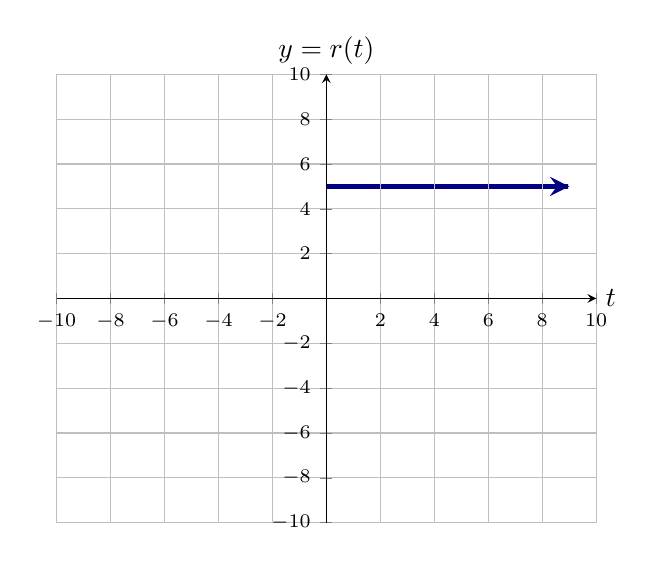
\begin{tikzpicture}
  \begin{axis}[
            domain=-10:10, ymax=10, xmax=10, ymin=-10, xmin=-10,
            axis lines =center, xlabel=$t$, ylabel={$y=r(t)$}, grid = major,
            ytick={-10,-8,-6,-4,-2,2,4,6,8,10},
            xtick={-10,-8,-6,-4,-2,2,4,6,8,10},
            yticklabels={$-10$,$-8$,$-6$,$-4$,$-2$,$2$,$4$,$6$,$8$,$10$}, 
            xticklabels={$-10$,$-8$,$-6$,$-4$,$-2$,$2$,$4$,$6$,$8$,$10$},
            ticklabel style={font=\scriptsize},
            every axis y label/.style={at=(current axis.above origin),anchor=south},
            every axis x label/.style={at=(current axis.right of origin),anchor=west},
            axis on top
          ]
          
          	
			\addplot [line width=2, penColor, smooth,samples=200,domain=(0:9),->] {5};
			%\addplot[color=penColor,fill=penColor,only marks,mark=*] coordinates{(0,0)};


  \end{axis}
\end{tikzpicture}
\end{image}



Since time is measured by the horizontal axis. our $distance = rate \times time$ calculation can be represented visually as the rectangular area under the rate curve.








\begin{image}
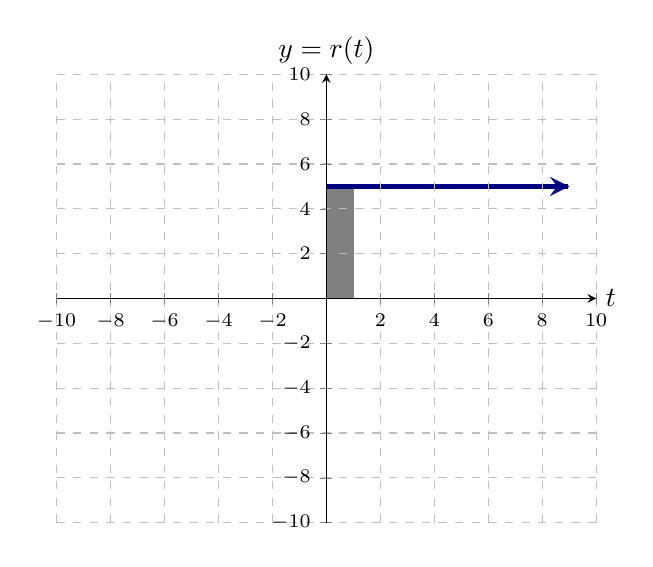
\begin{tikzpicture}
  \begin{axis}[
            domain=-10:10, ymax=10, xmax=10, ymin=-10, xmin=-10,
            axis lines =center, xlabel=$t$, ylabel={$y=r(t)$}, grid = major, grid style={dashed},
            ytick={-10,-8,-6,-4,-2,2,4,6,8,10},
            xtick={-10,-8,-6,-4,-2,2,4,6,8,10},
            yticklabels={$-10$,$-8$,$-6$,$-4$,$-2$,$2$,$4$,$6$,$8$,$10$}, 
            xticklabels={$-10$,$-8$,$-6$,$-4$,$-2$,$2$,$4$,$6$,$8$,$10$},
            ticklabel style={font=\scriptsize},
            every axis y label/.style={at=(current axis.above origin),anchor=south},
            every axis x label/.style={at=(current axis.right of origin),anchor=west},
            axis on top
          ]
          
          	

          	\draw[gray,fill=gray] (axis cs:0,0) -- (axis cs:0,5) -- (axis cs:1,5) -- (axis cs:1,0) -- (axis cs:0,0);
			\addplot [line width=2, penColor, smooth,samples=200,domain=(0:9),->] {5};

			%\addplot [name path=darkerA,domain=0:1,draw=none] {5};
			%\addplot [name path=darkerB,domain=0:1,draw=none] {0};
			%\addplot [blue!50!black!50] fill between[of=darkerA and darkerB];



			%\draw[gray,fill=gray] (axis cs:0,0) -- (axis cs:0,5) -- (axis cs:1,5) -- (axis cs:1,0) -- (axis cs:0,0);



  \end{axis}
\end{tikzpicture}
\end{image}


The area of the rectangle represents the distance travelled. \\

The height of the rectangle is the height of the graph, which is the value of the rate, $5 \, mph$.

The width of the rectangle is a time measurement. In the graph above, this is $1 \, hour$.

The area is height times width, which gives $area = 5 \, mph \times 1 \, hour = 5 \, miles$ \\



Let $D(t) = $ the accumulated miles travelled after $t \, hours$.

Graphically, this is the area of the rectangle below the graph from $0$ to $t$.  


\begin{model}

The formula would be $D(t) = \answer{5 t}$ miles.

\end{model}








\begin{image}
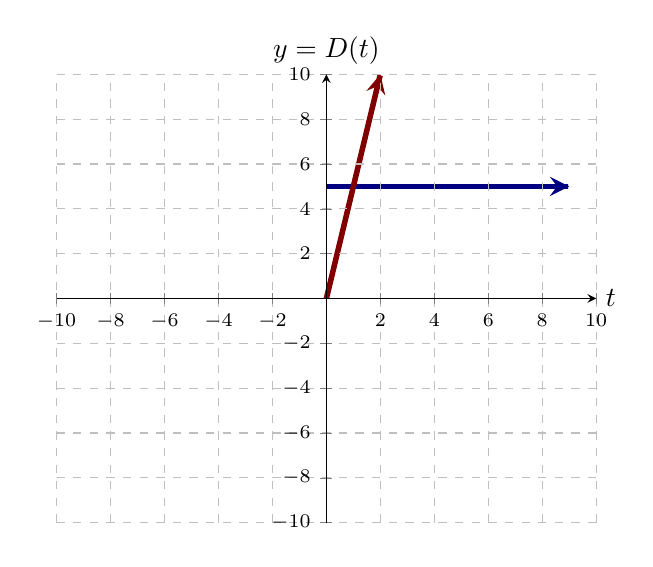
\begin{tikzpicture}
  \begin{axis}[
            domain=-10:10, ymax=10, xmax=10, ymin=-10, xmin=-10,
            axis lines =center, xlabel=$t$, ylabel={$y=D(t)$}, grid = major, grid style={dashed},
            ytick={-10,-8,-6,-4,-2,2,4,6,8,10},
            xtick={-10,-8,-6,-4,-2,2,4,6,8,10},
            yticklabels={$-10$,$-8$,$-6$,$-4$,$-2$,$2$,$4$,$6$,$8$,$10$}, 
            xticklabels={$-10$,$-8$,$-6$,$-4$,$-2$,$2$,$4$,$6$,$8$,$10$},
            ticklabel style={font=\scriptsize},
            every axis y label/.style={at=(current axis.above origin),anchor=south},
            every axis x label/.style={at=(current axis.right of origin),anchor=west},
            axis on top
          ]
          
          	

			\addplot [line width=2, penColor, smooth,samples=200,domain=(0:9), ->] {5};

			\addplot [line width=2, penColor2, smooth,samples=200,domain=(0:2), ->] {5*x};



  \end{axis}
\end{tikzpicture}
\end{image}



$D(t)$ is the accumulated distance travelled in $t \, hours$, which makes $r(t)$ its derivative.

\[    D'(t) = r(t)        \]


\[    (5 t)' = 5     \]





$\blacktriangleright$ \textbf{A Linear Rate}



This time our rate function is a linear function: $r(t) = 2 t$. \\

Our car goes faster as it goes farther.






\begin{image}
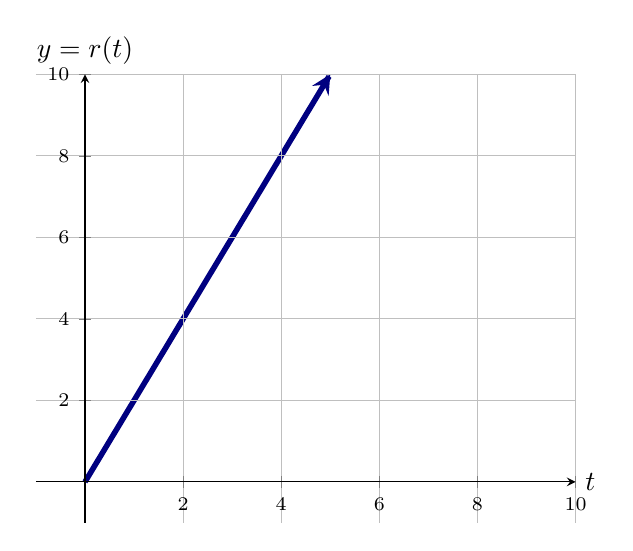
\begin{tikzpicture}
  \begin{axis}[
            domain=-1:10, ymax=10, xmax=10, ymin=-1, xmin=-1,
            axis lines =center, xlabel=$t$, ylabel={$y=r(t)$}, grid = major,
            ytick={2,4,6,8,10},
            xtick={2,4,6,8,10},
            yticklabels={$2$,$4$,$6$,$8$,$10$}, 
            xticklabels={$2$,$4$,$6$,$8$,$10$},
            ticklabel style={font=\scriptsize},
            every axis y label/.style={at=(current axis.above origin),anchor=south},
            every axis x label/.style={at=(current axis.right of origin),anchor=west},
            axis on top
          ]
          
          	
			\addplot [line width=2, penColor, smooth,samples=200,domain=(0:5),->] {2*x};
			%\addplot[color=penColor,fill=penColor,only marks,mark=*] coordinates{(0,0)};


  \end{axis}
\end{tikzpicture}
\end{image}



$Distance$ is still represented visually as the area under the rate curve.


The area is a triangle this time. 




\begin{image}
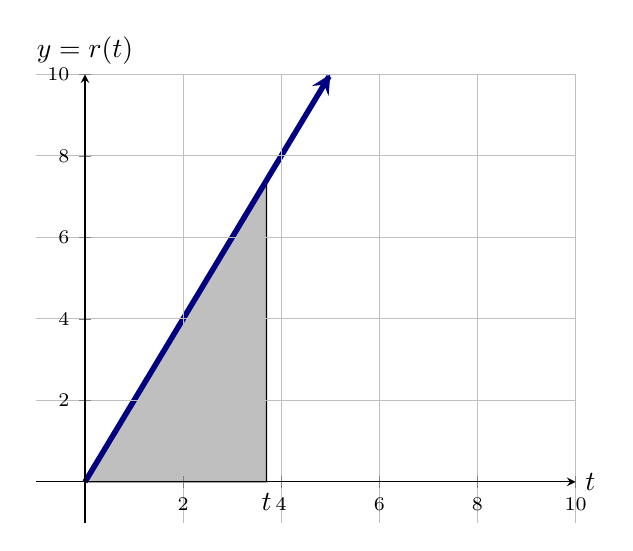
\begin{tikzpicture}
  \begin{axis}[
            domain=-1:10, ymax=10, xmax=10, ymin=-1, xmin=-1,
            axis lines =center, xlabel=$t$, ylabel={$y=r(t)$}, grid = major,
            ytick={2,4,6,8,10},
            xtick={2,4,6,8,10},
            yticklabels={$2$,$4$,$6$,$8$,$10$}, 
            xticklabels={$2$,$4$,$6$,$8$,$10$},
            ticklabel style={font=\scriptsize},
            every axis y label/.style={at=(current axis.above origin),anchor=south},
            every axis x label/.style={at=(current axis.right of origin),anchor=west},
            axis on top
          ]
          
          	\draw[black,fill=lightgray] (axis cs:0,0) -- (axis cs:3.7,7.4) -- (axis cs:3.7,0) -- (axis cs:0,0);
			\addplot [line width=2, penColor, smooth,samples=200,domain=(0:5),->] {2*x};
			%\addplot[color=penColor,fill=penColor,only marks,mark=*] coordinates{(0,0)};
			\node at (axis cs:3.7,-0.5) [black] {$t$};


  \end{axis}
\end{tikzpicture}
\end{image}



 Over the interval $[0,t]$, the area is $D(t) = \frac{1}{2} \cdot t \cdot (2 t) = t^2$



$D(t) = t^2$ is the accumulated distance travelled in $t \, hours$, which makes $2 t$ its derivative.



\[    (t^2)' = 2 t     \]












\begin{image}
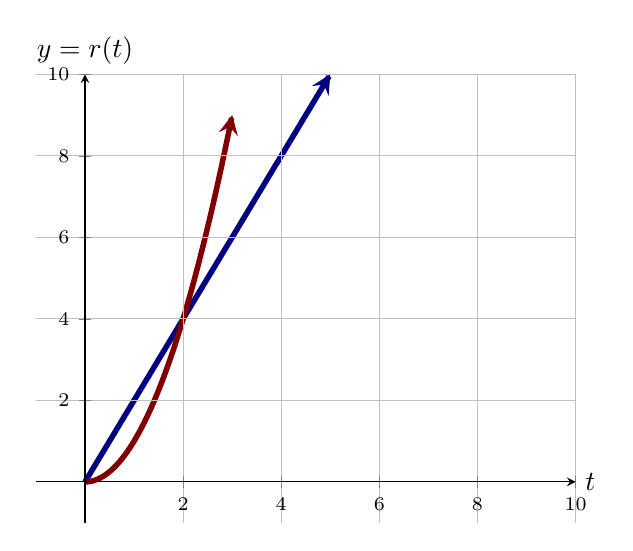
\begin{tikzpicture}
  \begin{axis}[
            domain=-1:10, ymax=10, xmax=10, ymin=-1, xmin=-1,
            axis lines =center, xlabel=$t$, ylabel={$y=r(t)$}, grid = major,
            ytick={2,4,6,8,10},
            xtick={2,4,6,8,10},
            yticklabels={$2$,$4$,$6$,$8$,$10$}, 
            xticklabels={$2$,$4$,$6$,$8$,$10$},
            ticklabel style={font=\scriptsize},
            every axis y label/.style={at=(current axis.above origin),anchor=south},
            every axis x label/.style={at=(current axis.right of origin),anchor=west},
            axis on top
          ]
          
          	
			\addplot [line width=2, penColor, smooth,samples=200,domain=(0:5),->] {2*x};
			\addplot [line width=2, penColor2, smooth,samples=200,domain=(0:3),->] {x^2};
			%\addplot[color=penColor,fill=penColor,only marks,mark=*] coordinates{(0,0)};


  \end{axis}
\end{tikzpicture}
\end{image}




























\section*{Accumulation}



Below is the graph of $y = p(k) = -k^2 + 7$, approximated with

\[
L(k) = 
\begin{cases}
  4(k+2)+3       &          \text{ on } \,     \left(-3, -\frac{3}{2}\right]   \\
  2(k+1)+6       &          \text{ on } \,     \left(-\frac{3}{2}, -\frac{1}{2}\right]   \\
  7              &          \text{ on } \,     \left(-\frac{1}{2}, \frac{1}{2}\right]   \\
  -2(k-1)+6      &          \text{ on } \,     \left(\frac{1}{2}, \frac{3}{2}\right]   \\
  -4(k-2)+3      &          \text{ on } \,     \left(\frac{3}{2}, 3\right)   
\end{cases}
\]


$L(k)$ is a piecewise linear function, which means we can calculate area using rectangles and triangles.


\begin{image}
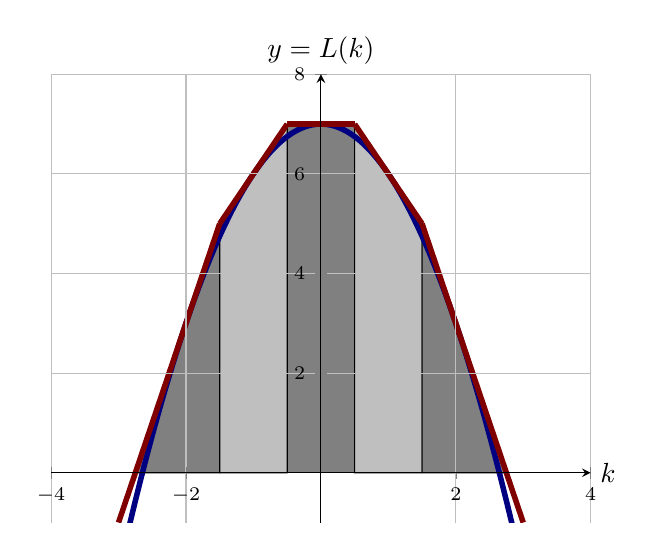
\begin{tikzpicture}
  \begin{axis}[
            domain=-4:4, ymax=8, xmax=4, ymin=-1, xmin=-4,
            axis lines =center, xlabel=$k$, ylabel={$y=L(k)$}, grid = major,
            ytick={2,4,6,8},
            xtick={-4,-2,2,4},
            yticklabels={$2$,$4$,$6$,$8$}, 
            xticklabels={$-4$,$-2$,$2$,$4$},
            ticklabel style={font=\scriptsize},
            every axis y label/.style={at=(current axis.above origin),anchor=south},
            every axis x label/.style={at=(current axis.right of origin),anchor=west},
            axis on top
          ]
          
          	\draw[black,fill=gray] (axis cs:-2.75,0) -- (axis cs:-1.5,5) -- (axis cs:-1.5,0) -- (axis cs:-2.75,0);
          	\draw[black,fill=lightgray] (axis cs:-1.5,0) -- (axis cs:-1.5,5) -- (axis cs:-0.5,7) -- (axis cs:-0.5,0) -- (axis cs:-1.5,0);
          	\draw[black,fill=gray] (axis cs:-0.5,0) -- (axis cs:-0.5,7) -- (axis cs:0.5,7) -- (axis cs:0.5,0) -- (axis cs:-0.5,0);
          	\draw[black,fill=lightgray] (axis cs:1.5,0) -- (axis cs:1.5,5) -- (axis cs:0.5,7) -- (axis cs:0.5,0) -- (axis cs:1.5,0);
          	\draw[black,fill=gray] (axis cs:2.75,0) -- (axis cs:1.5,5) -- (axis cs:1.5,0) -- (axis cs:2.75,0);
          	
			\addplot [line width=2, penColor, smooth,samples=200,domain=(-4:4),<->] {-(x^2)+7};
			%\addplot[color=penColor,fill=penColor,only marks,mark=*] coordinates{(0,0)};
			\addplot [line width=2, penColor2, smooth,samples=200,domain=(-3:-1.5)] {4*(x+2)+3};
			\addplot [line width=2, penColor2, smooth,samples=200,domain=(-1.5:-0.5)] {2*(x+1)+6};
			\addplot [line width=2, penColor2, smooth,samples=200,domain=(-0.5:0.5)] {7};
			\addplot [line width=2, penColor2, smooth,samples=200,domain=(0.5:1.5)] {-2*(x-1)+6};
			\addplot [line width=2, penColor2, smooth,samples=200,domain=(1.5:3)] {-4*(x-2)+3};

  \end{axis}
\end{tikzpicture}
\end{image}


The shaded regions are made of triangles, trapezoids, and rectangles.  And, we know their formulas from Geometry class.


\begin{center}

area = triangle + trapezoid + rectangle + trapezoid + triangle
\end{center}



\[ \text{Area} = \frac{1}{2} \cdot 1.25 \cdot L(-1.5) + \frac{1}{2} \cdot (L(-1.5) + L(-0.5)) \cdot 1 + 1 \cdot L(0.5) + \frac{1}{2} \cdot (L(1.5) + L(0.5)) \cdot 1  +    \frac{1}{2} \cdot 1.25 \cdot L(1.5)    \]



\[ \text{Area} = \frac{1}{2} \cdot 1.25 \cdot 5 + \frac{1}{2} \cdot 12 \cdot 1 + 1 \cdot 7 + \frac{1}{2} \cdot 12 \cdot 1  +    \frac{1}{2} \cdot 1.25 \cdot 5    \]


\[ \text{Area} = 25.25    \]


This is the area under $y = L(x)$, so it is the approximate area under $y = p(k) = -k^2 + 7$ from $k = -3$ to $k = 3$.


































\begin{center}
\textbf{\textcolor{green!50!black}{ooooo-=-=-=-ooOoo-=-=-=-ooooo}} \\

more examples can be found by following this link\\ \link[More Examples of Approximate Behavior]{https://ximera.osu.edu/csccmathematics/precalculus/precalculus/nearEquivalentBehavior/examples/exampleList}

\end{center}





\end{document}
